\documentclass[a4paper, 11pt]{article} % Font size (can be 10pt, 11pt or 12pt) and paper size (remove a4paper for US letter paper)

\usepackage[protrusion=true,expansion=true]{microtype} % Better typography
\usepackage{graphicx} % Required for including pictures
\usepackage{hyperref}
\usepackage{float}

 \usepackage{natbib}

\usepackage{mathpazo} % Use the Palatino font
\usepackage[T1]{fontenc} % Required for accented characters
\linespread{1.05} % Change line spacing here, Palatino benefits from a slight increase by default

\makeatletter
\renewcommand\@biblabel[1]{\textbf{#1.}} % Change the square brackets for each bibliography item from '[1]' to '1.'
\renewcommand{\@listI}{\itemsep=0pt} % Reduce the space between items in the itemize and enumerate environments and the bibliography

\renewcommand{\maketitle}{ % Customize the title - do not edit title and author name here, see the TITLE block below
\begin{flushright} % Right align
{\LARGE\@title} % Increase the font size of the title

\vspace{50pt} % Some vertical space between the title and author name

{\large\@author} % Author name
\\\@date % Date

\vspace{40pt} % Some vertical space between the author block and abstract
\end{flushright}
}

%----------------------------------------------------------------------------------------
%	TITLE
%----------------------------------------------------------------------------------------

\title{\textbf{PhyloGeoTool}\\ % Title
User Reference Manual} % Subtitle

\author{\textsc{Ewout Vanden Eynden, Pieter Libin, Kristof Theys, anderen, Guy Baele} % Author
\\{\textit{Rega Institute for Medical Research, KU Leuven}}} % Institution

\date{August 2016} % Date

%----------------------------------------------------------------------------------------

\begin{document}
\maketitle % Print the title section

\vspace{30pt} % Some vertical space between the abstract and first section

%------------------------------------------------
\tableofcontents
\newpage

This document provides additional information on how to use an instance of the PhyloGeoTool. Most users will access a publically (or privately) accessible instance of the PhyloGeoTool. An example of a publically available instance of the PhyloGeoTool that aims to serve a large HIV cohort can be found at \url{http://regatools.med.kuleuven.be/phylogeotool/PhyloGeoTool}.\\
It is however also possible to install your own instance of the PhyloGeoTool, for this, we refer you to the installation manual (TODO: add link).

\section{Getting started}

PhyloGeoTool implements a visual method to explore large phylogenetic trees and to depict characteristics of strains and clades, including their geographic context, in an interactive way.
The tool also provides the possibility to insert new virus strains into the existing phylogenetic tree, allowing users to gain insight in the placement of such new strains without the need to reconstruct the phylogeny.

A particular PhyloGeoTool instance can be used by navigating the browser to the URL at which this instance has been deployed. For example, the aforementioned public HIV instance of the PhyloGeoTool is deployed at \url{http://regatools.med.kuleuven.be/phylogeotool/PhyloGeoTool}, and thus, you should navigate your browser to this exact URL.\\
TODO: explaining what instances are all about, is easier if you can mention more than 1 instance. Perhaps Lize will have a HCV/DENV instance ready soon, that we can add here, but maybe we should both deploy the EuResist and PT tool, such that we can list them in this section.\\
Note that any browser (Chrome, Firefox, Internet Explorer) should do, if you experience any problems with your browser, please contact us (TODO: link to the contact section).


\section{Core user interface and functionality}




\begin{figure}[H]
\centering
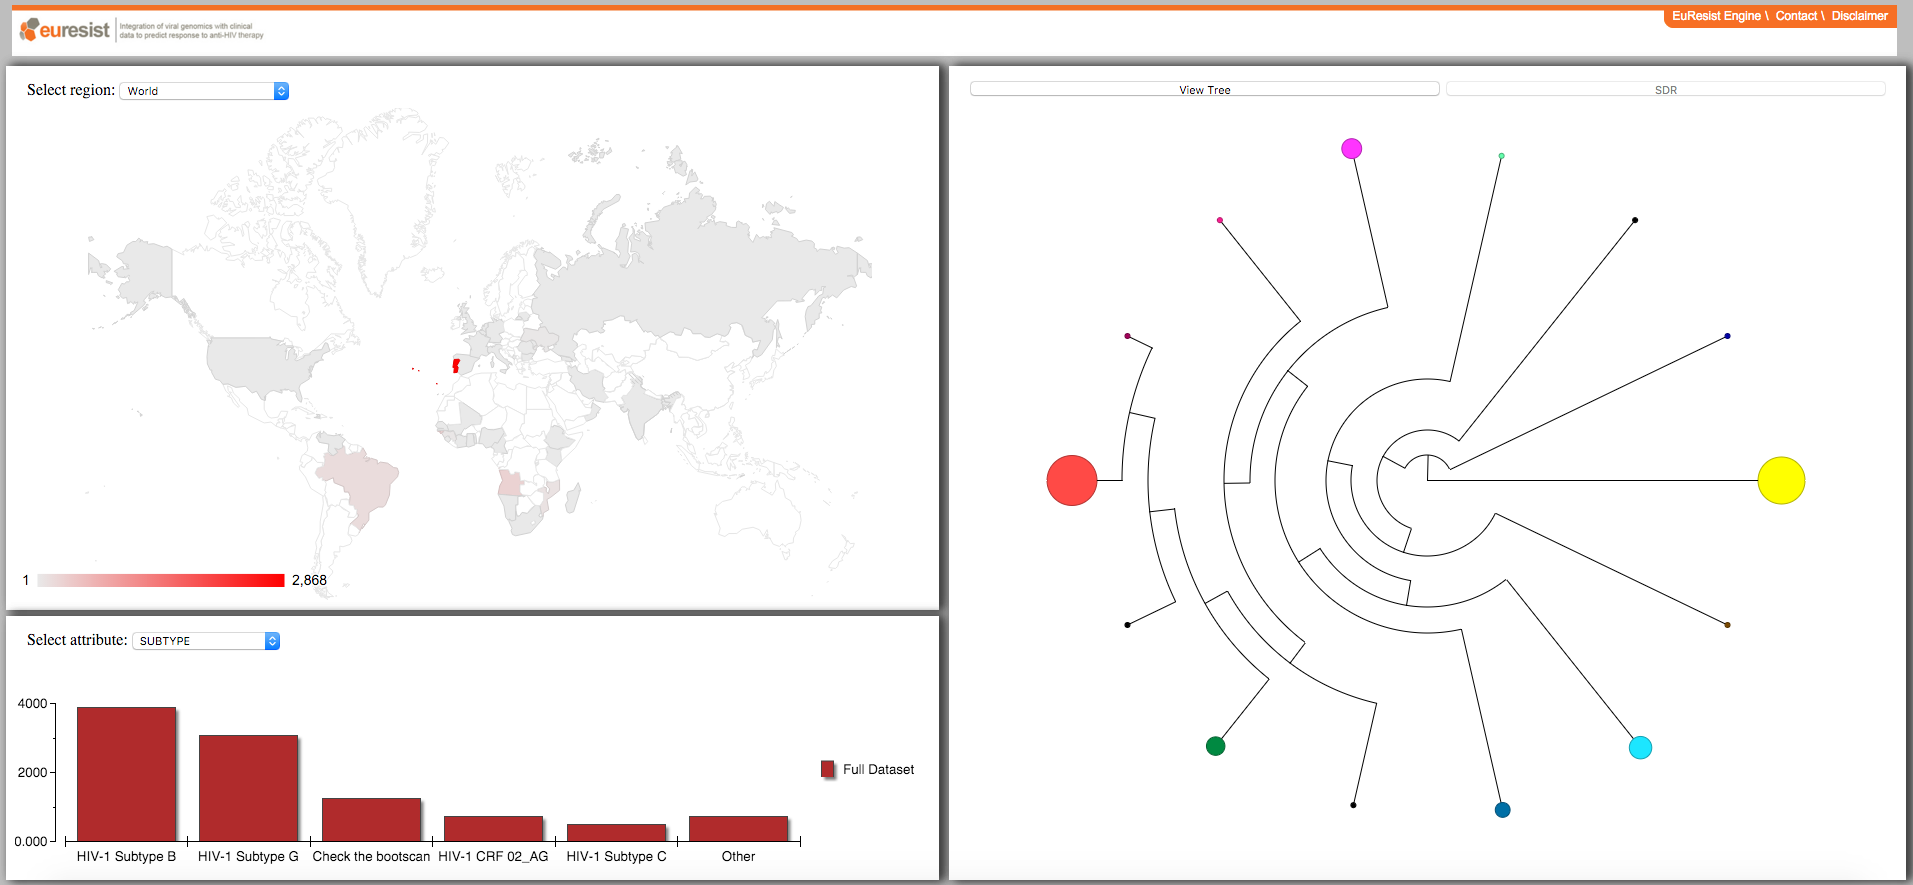
\includegraphics[width=400pt, height=400pt, keepaspectratio=true]{images/initial_view.PNG}
\caption{Start and main view of the PhyloGeoTool. By default, the panel on the upper left shows a map that depics the geographical distribution of the sequences of the relevant phylogeny, the lower left panel shows bar chart that depicts the value distribution for one of the sequence attributes, and the right panel shows a top-level view of the clustering of the tree, as determined by our clustering algorithm (TODO: add reference to our paper).}
\label{fig:initial_view}
\end{figure}

The tool is divided into different panels: 
\begin{itemize}
  \item The top left panel shows a map where each country is colored according to a gradient, where a darker color signifies that more sequences are originating from this country. A drop down box allows you to select the geographic region on which you want to focus (e.g. Europe, North-America, \ldots).
  \item The bottom left panel shows a bar chart which shows a certain attribute (i.e. characteristic) from all sequences currently visualized in the tree-panel on the right. A drop down box allows you to select the attribute to be plotted on the bar chart. The attributes available for selection depend on the attributes made available by the PhyloGeoTool instance.
  \item The right panel initially shows the root of the clustered phylogeny. A button allows you to visualise the phylogenetic tree in its entirety, colored according to the clustering scheme.
\end{itemize}

\subsubsection{Hover over node in clustered phylogeny}
\begin{figure}[H]
\centering
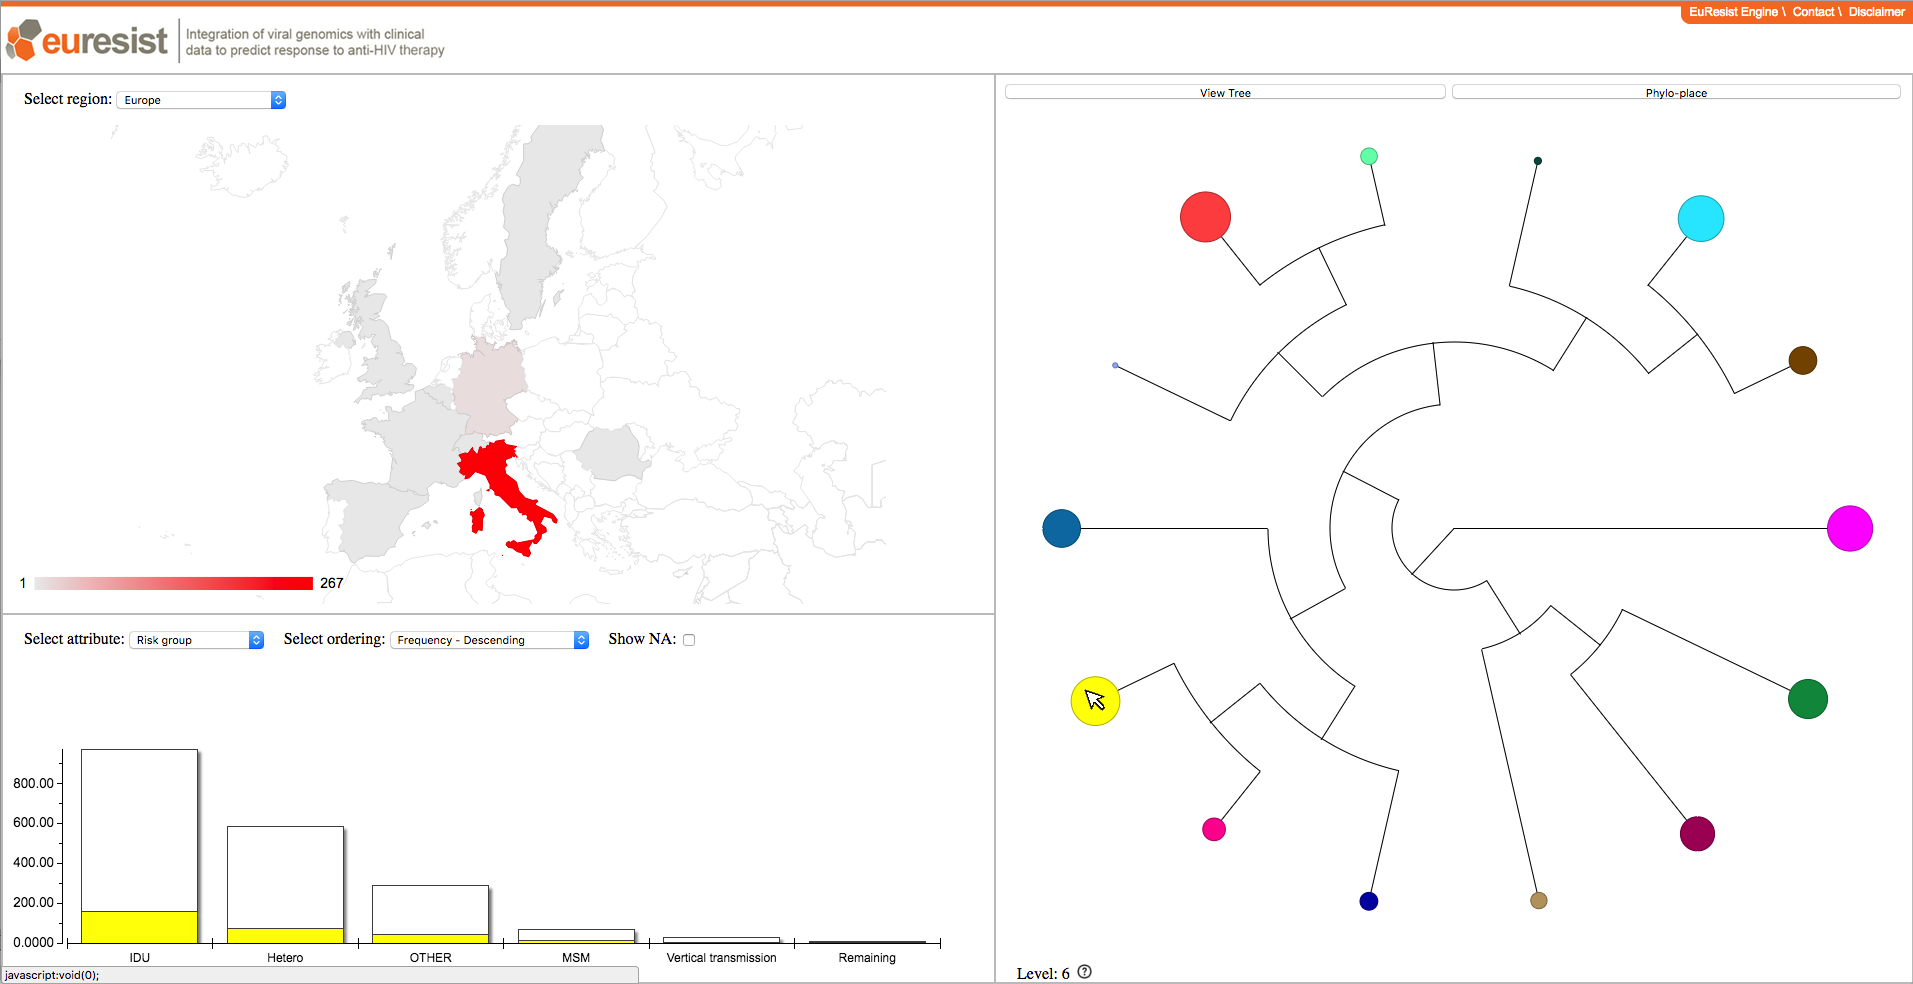
\includegraphics[width=400pt, height=400pt, keepaspectratio=true]{images/hover_node.PNG}
\caption{Hovering over a node in the cluster phylogeny}
\label{fig:hover_node}
\end{figure}

When a node in the cluster phylogeny is hoovered, both the attribute bar chart and the map are updated. The attribute bar chart will be extended (i.e. extra bars) with the data that is located in the hovered cluster. The map will show the geographic distribution of the sequences found in the hovered cluster only.
\\
When you click on a node in the clustered phylogeny, you will navigate to the clustering of this particular node (i.e. you will zoom in on the node on the clustered phylogeny).
A counter on the bottom left of the cluster panel keeps track of the depth of your navigation. As you can visit a cluster node by clicking it, you can go back to into your navigational path by using the browser 'Back' button.
\\
Additionally, the URL encodes the level of descent in the clustered phylogeny. An URL can thus be bookmarked or shared to go back at the exact location in the clustered phylogeny.\\ 
TODO: is URL decoding already implemented? (see issue #31)

\subsection{Change region}
\begin{figure}[H]
\centering
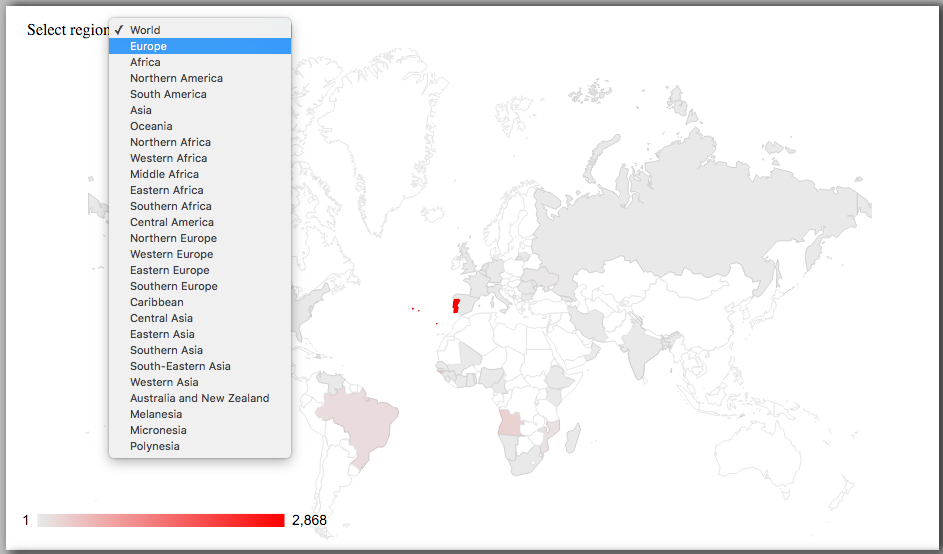
\includegraphics[width=400pt, height=400pt, keepaspectratio=true]{images/change_country.PNG}
\caption{Change the region in the drop down box}
\label{fig:change_region}
\end{figure}
You can select your geographical region of interest in the drop down box on top of the map (see fig. \ref{fig:change_region}). 

\subsubsection{Change attribute}
\begin{figure}[H]
\centering
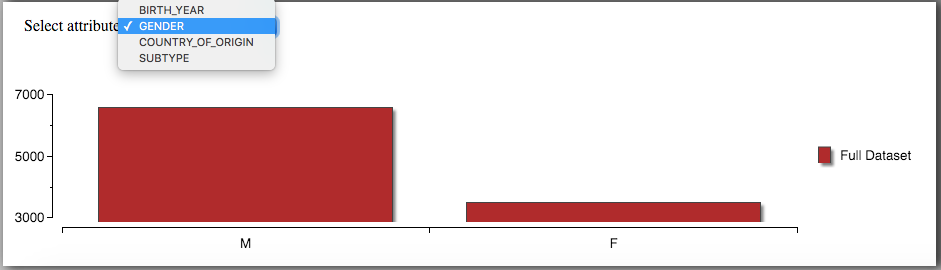
\includegraphics[width=400pt, height=400pt, keepaspectratio=true]{images/change_attr.PNG}
\caption{Change the attribute in the drop down box}
\label{fig:change_attr}
\end{figure}
When you change the attribute by selecting a new value in the drop down box on top of the bar chart (see fig. \ref{fig:change_attr}), the chart will update and now only show data for this specific newly selected attribute.

\subsubsection{View Tree}
\begin{figure}[H]
\centering
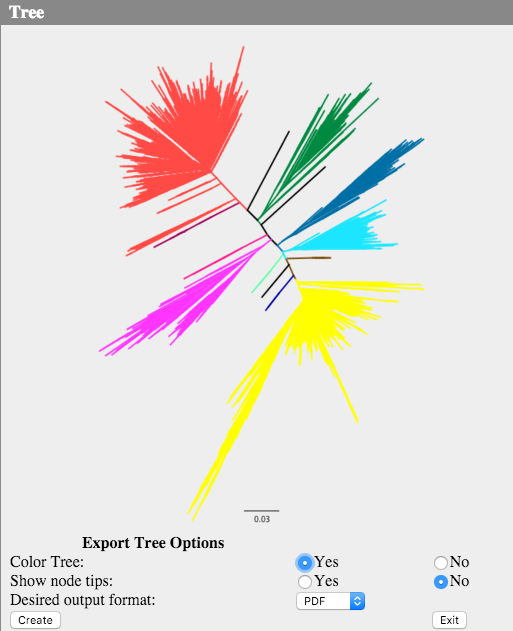
\includegraphics[width=400pt, height=400pt, keepaspectratio=true]{images/view_tree.PNG}
\caption{Tree visualization in FigTree}
\label{fig:view_tree}
\end{figure}
When the 'View Tree' button on top of the circular phylogenetic tree representation is clicked, a popup window will appear such as in fig. \ref{fig:view_tree} where the tree is shown as a radial tree such as it is represented in FigTree. The different clusters get different colours. The colours in the radial tree representation correspond to the colours in the circular tree representation.
\\
In addition to the visualisation of the tree, export options are available. The user can select if he/she wants the tree to be coloured, if the node tips should be shown and in which format the tree will be exported. 

\subsection{PPlacer}
pplacer is a software package for phylogenetic placement and subsequent visualization \citep{Matsen2010}.
Phylogenetic placement allows to insert/place unknown query sequences onto an existing phylogenetic tree via a reference alignment and uses techniques from likelihood-based phylogenetic inference to do so.
As such, pplacer features calculation of the posterior probability of the placement on an edge, which is a statistically rigorous way of quantifying uncertainty on an edge-by-edge basis.

PhyloGeoTool focuses on using pplacer to position additional sequences onto a previously reconstructed phylogenetic tree.
To do so, select PPlacer in the clustering window; there are two ways to add a new sequence to the tree:
\begin{itemize}
\item Paste the nucleotide sequence you'd like to add in the presented window.
\item Choose a Fasta file containing the nucleotide sequence using the file chooser.
\item Fasta files containing multiple sequences are allowed up to a total of MAX sequences, which will be placed sequentially into the phylogenetic tree.
\end{itemize}



\section{Example: exploring an HIV-1 data set}

In this section, we provide an example application of the PhyloGeoTool on HIV-1 using data available within the EuResist Integrated Data Base \citep{Zazzi2012}. 
This database contains virus genotypes, clinical responses and epidemiological markers of more than 66.000 patients from 12 different countries.

\bibliographystyle{natbib}%%%%natbib.sty
\bibliography{References}%%%refs.bib

\end{document}
